\section[Xbase]{Implementation in Xbase}

\begin{frame}
  \frametitle{Implementation in Xbase}
  \tableofcontents[currentsection]
\end{frame}
  
\begin{frame}[fragile,allowframebreaks]
  \frametitle{Implementation in Xbase}
  \begin{itemize}
    \item Attributes of entities refer to Java elements
    \item Infer Java type for Entities and Forms with
    \emph{JvmModelInferrer}
  \end{itemize}
  
  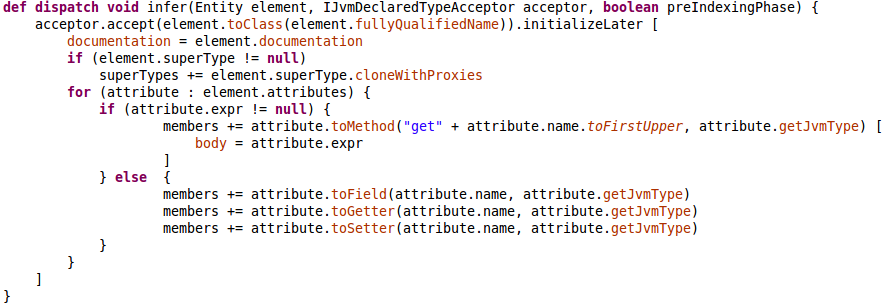
\includegraphics[width=\textwidth]{img/xbase-infer.png}  
 
\begin{footnotesize}
% Generator: GNU source-highlight, by Lorenzo Bettini, http://www.gnu.org/software/src-highlite
\begin{tabular}[t]{l}
\noindent
\mbox{}\textbf{\textcolor{Blue}{def}}\ \textbf{\textcolor{Blue}{dispatch}}\ \textcolor{ForestGreen}{void}\ \textbf{\textcolor{Black}{infer}}\textcolor{BrickRed}{(}Entity\ element\textcolor{BrickRed}{,}\ IJvmDeclaredTypeAcceptor\ acceptor\textcolor{BrickRed}{,}\ \textcolor{ForestGreen}{boolean}\ preIndexingPhase\textcolor{BrickRed}{)}\ \textcolor{Red}{\{} \\
\mbox{}\ \ \ \ acceptor\textcolor{BrickRed}{.}\textbf{\textcolor{Black}{accept}}\textcolor{BrickRed}{(}element\textcolor{BrickRed}{.}\textbf{\textcolor{Black}{toClass}}\textcolor{BrickRed}{(}element\textcolor{BrickRed}{.}fullyQualifiedName\textcolor{BrickRed}{)).}initializeLater\ \textcolor{BrickRed}{[} \\
\mbox{}\ \ \ \ \ \ \ \ documentation\ \textcolor{BrickRed}{=}\ element\textcolor{BrickRed}{.}documentation \\
\mbox{}\ \ \ \ \ \ \ \ \textbf{\textcolor{Blue}{if}}\ \textcolor{BrickRed}{(}element\textcolor{BrickRed}{.}superType\ \textcolor{BrickRed}{!=}\ \textbf{\textcolor{Blue}{null}}\textcolor{BrickRed}{)} \\
\mbox{}\ \ \ \ \ \ \ \ \ \ \ \ superTypes\ \textcolor{BrickRed}{+=}\ element\textcolor{BrickRed}{.}superType\textcolor{BrickRed}{.}cloneWithProxies \\
\mbox{}\ \ \ \ \ \ \ \ \textbf{\textcolor{Blue}{for}}\ \textcolor{BrickRed}{(}attribute\ \textcolor{BrickRed}{:}\ element\textcolor{BrickRed}{.}attributes\textcolor{BrickRed}{)}\ \textcolor{Red}{\{} \\
\mbox{}\ \ \ \ \ \ \ \ \ \ \ \ \textbf{\textcolor{Blue}{if}}\ \textcolor{BrickRed}{(}attribute\textcolor{BrickRed}{.}expr\ \textcolor{BrickRed}{!=}\ \textbf{\textcolor{Blue}{null}}\textcolor{BrickRed}{)}\ \textcolor{Red}{\{} \\
\mbox{}\ \ \ \ \ \ \ \ \ \ \ \ \ \ \ \ \ \ \ \ members\ \textcolor{BrickRed}{+=}\ attribute\textcolor{BrickRed}{.}\textbf{\textcolor{Black}{toMethod}}\textcolor{BrickRed}{(}\texttt{\textcolor{Red}{"{}get"{}}}\ \textcolor{BrickRed}{+}\ attribute\textcolor{BrickRed}{.}name\textcolor{BrickRed}{.}toFirstUpper\textcolor{BrickRed}{,}\ attribute\textcolor{BrickRed}{.}getJvmType\textcolor{BrickRed}{)}\ \textcolor{BrickRed}{[} \\
\mbox{}\ \ \ \ \ \ \ \ \ \ \ \ \ \ \ \ \ \ \ \ \ \ \ \ body\ \textcolor{BrickRed}{=}\ attribute\textcolor{BrickRed}{.}expr \\
\mbox{}\ \ \ \ \ \ \ \ \ \ \ \ \ \ \ \ \ \ \ \ \textcolor{BrickRed}{]} \\
\mbox{}\ \ \ \ \ \ \ \ \ \ \ \ \textcolor{Red}{\}}\ \textbf{\textcolor{Blue}{else}}\ \ \textcolor{Red}{\{} \\
\mbox{}\ \ \ \ \ \ \ \ \ \ \ \ \ \ \ \ \ \ \ \ members\ \textcolor{BrickRed}{+=}\ attribute\textcolor{BrickRed}{.}\textbf{\textcolor{Black}{toField}}\textcolor{BrickRed}{(}attribute\textcolor{BrickRed}{.}name\textcolor{BrickRed}{,}\ attribute\textcolor{BrickRed}{.}getJvmType\textcolor{BrickRed}{)} \\
\mbox{}\ \ \ \ \ \ \ \ \ \ \ \ \ \ \ \ \ \ \ \ members\ \textcolor{BrickRed}{+=}\ attribute\textcolor{BrickRed}{.}\textbf{\textcolor{Black}{toGetter}}\textcolor{BrickRed}{(}attribute\textcolor{BrickRed}{.}name\textcolor{BrickRed}{,}\ attribute\textcolor{BrickRed}{.}getJvmType\textcolor{BrickRed}{)} \\
\mbox{}\ \ \ \ \ \ \ \ \ \ \ \ \ \ \ \ \ \ \ \ members\ \textcolor{BrickRed}{+=}\ attribute\textcolor{BrickRed}{.}\textbf{\textcolor{Black}{toSetter}}\textcolor{BrickRed}{(}attribute\textcolor{BrickRed}{.}name\textcolor{BrickRed}{,}\ attribute\textcolor{BrickRed}{.}getJvmType\textcolor{BrickRed}{)} \\
\mbox{}\ \ \ \ \ \ \ \ \ \ \ \ \textcolor{Red}{\}} \\
\mbox{}\ \ \ \ \ \ \ \ \textcolor{Red}{\}} \\
\mbox{}\ \ \ \ \textcolor{BrickRed}{]} \\
\mbox{}\textcolor{Red}{\}}
\end{tabular}

\end{footnotesize}

%   \begin{verbatim}
%     	def dispatch void infer(Entity element, IJvmDeclaredTypeAcceptor acceptor, boolean preIndexingPhase) {
%    		acceptor.accept(element.toClass(element.fullyQualifiedName)).initializeLater [
% 			documentation = element.documentation
% 			if (element.superType != null)
% 				superTypes += element.superType.cloneWithProxies
% 		    for (attribute : element.attributes) {
% 		    	if (attribute.expr != null) {
% 						members += attribute.toMethod("get" + attribute.name.toFirstUpper, attribute.getJvmType) [
% 			        		body = attribute.expr
% 		        		]
% 		        } else  {
% 		            	members += attribute.toField(attribute.name, attribute.getJvmType)
% 			            members += attribute.toGetter(attribute.name, attribute.getJvmType)
% 			            members += attribute.toSetter(attribute.name, attribute.getJvmType)
% 		        }
% 		    }
%    		]
%    	}
% 
%  	def dispatch void infer(Form form, IJvmDeclaredTypeAcceptor acceptor, boolean preIndexingPhase) {
%    		acceptor.accept(form.toClass(form.fullyQualifiedName)).initializeLater [
% 			documentation = form.documentation
% 		    for (widget: form.widgets) {
% 		    	if (widget.validate != null && widget.attr != null) {
% 		    		members += widget.toMethod('validate'+widget.attr.name.toFirstUpper, form.newTypeRef(Boolean::TYPE)) [
% 		    			parameters += widget.toParameter("it", form.entity.getJvmType)
% 		    			parameters += widget.toParameter("widgetcontent", widget.attr.getJvmType)
% 		    			body = widget.validate
% 		    		]
% 		    	}
% 		    }   		 	
%    		]
%    	}
%   \end{verbatim}
  
\end{frame}